\documentclass{magnolia}

\magtex{tex_driver={pdftex},
        tex_packages={xypic,slashbox,tikz,pgfplots,epigraph}}
\magfiche{document_nom={Cours sur les équations différentielles},
          auteur_nom={François Fayard},
          auteur_mail={fayard.prof@gmail.com}}
\magcours{cours_matiere={maths},
          cours_niveau={mpsi},
          cours_chapitre_numero={6},
          cours_chapitre={Équations différentielles}}
\magmisenpage{misenpage_presentation={tikzvelvia},
          misenpage_format={a4},
          misenpage_nbcolonnes={1},
          misenpage_preuve={non},
          misenpage_sol={non}}
\maglieudiff{}
\magprocess

\begin{document}

%BEGIN_BOOK
\setlength\epigraphwidth{.65\textwidth}
\epigraph{\og J'entends et j'oublie. Je vois et je me souviens. Je fais et je comprends.\fg}{--- \textsc{Confucius (551--479 AV J.C.)}}
\setlength\epigraphwidth{.35\textwidth}
\epigraph{\og Les calculs sont pas bons, Kevin~!\fg}{--- \textsc{Inès Reg (2019)}}

\magtoc

\vspace{2ex}
Dans ce chapitre, $\K$ désignera l'un des corps $\R$ ou $\C$.

\section{Équation différentielle linéaire du premier ordre}

\begin{definition}
Soit $a,b,c:I\to\K$ des fonctions définies sur un intervalle $I$. On appelle
solution sur $I$ de l'équation différentielle linéaire du premier ordre $a y'+b y=c$, toute
fonction $y:I\to\K$, dérivable sur $I$, telle que
\[\forall t\in I\qsep a(t)y'(t)+b(t)y(t)=c(t).\]
On dit que l'équation est \emph{résolue} lorsque $a$ ne s'annule pas et qu'elle est
\emph{homogène} lorsque la fonction $c$ est nulle.
\end{definition}

\begin{remarqueUnique}
\remarque Lorsque l'équation est résolue, on peut l'écrire sous la forme
  \[\forall t\in I\qsep y'(t)=F(y(t),t)\]
  où $F$ est une fonction de $\K\times I$ dans $\K$.
\end{remarqueUnique}

\subsection{Équation différentielle homogène}


\begin{sol}
\begin{victor}
\begin{eqnarray*}
y'+\lambda y=0 &\Longleftrightarrow& \forall x \in \R, y'(x)+\lambda y(x)=0 \\
&\Longleftrightarrow& \forall x \in \R, (y'(x)+\lambda y(x))e^{\lambda x}=0 \\
&\Longleftrightarrow& \forall x \in \R, \frac{d}{dx}\p{y(x)e^{\lambda x}}=0 \\
&\Longleftrightarrow& \exists C\in \R, \forall x \in \R, y(x)e^{\lambda x}=C \\
&\Longleftrightarrow& \exists C\in \R, \forall x \in \R, y(x)=Ce^{-\lambda x}.
\end{eqnarray*}
\end{victor}
\end{sol}


\begin{proposition}[utile=-3]
Soit $a:I\to\K$ une fonction continue sur un intervalle $I$. Si $A$ est
une primitive de $a$ sur $I$, les solutions de l'équation différentielle
\[\forall t\in I \qsep y'(t)+a(t)y(t)=0\]
sont les fonctions
\[\dspappli{y_\lambda}{I}{\K}{t}{\lambda \e^{-A(t)}}\]
où $\lambda\in\K$.
\end{proposition}

\begin{preuve}
\begin{francois}
Soit $I$ un intervalle et $a:I\to\R$ une fonction continue. On souhaite résoudre l'équation différentielle
\[(E)\qquad\forall t\in I\qsep y'(t)+a(t)y(t)=0.\]
Soit $y:I\to\R$ une fonction dérivable quelconque. Alors
\begin{eqnarray*}
\text{$y$ est solution de $(E)$}
&\ssi& \forall t\in I\qsep y'(t)+a(t)y(t)=0\\
&\ssi& \forall t\in I\qsep y'(t)\e^{A(t)}+a(t)y(t)\e^{A(t)}=0\\
&    & \text{où $A$ est une primitive de la fonction continue $a$}\\
&\ssi& \forall t\in I\qsep \frac{{\rm d}}{{\rm d}t}\p{y(t)\e^{A(t)}}=0\\
&\ssi& \exists \lambda\in\R\qsep\forall t\in I\qsep y(t)\e^{A(t)}=\lambda\\
&    & \text{car $I$ est un intervalle}\\
&\ssi& \exists \lambda\in\R\qsep\forall t\in I\qsep y(t)=\lambda\e^{-A(t)}
\end{eqnarray*}
Les solutions réelles de $(E)$ sont donc les fonctions $t\mapsto \lambda \e^{-A(t)}$
où $\lambda\in\R$.
\end{francois}
\begin{victor}
\begin{eqnarray*}
u \text{ solution de } (E_0) \text{ sur } I&\Longleftrightarrow & u'+au=0 \\
&\Longleftrightarrow & (u'+au)\e^A=0 \qquad\text{ car } \e^A\neq 0, \forall x \in I \\
&\Longleftrightarrow &(u\e^A)'=0\\
&\Longleftrightarrow & \exists c\in \K \text{ tel que } ue^A=c\\
&\Longleftrightarrow & \exists c\in \K \text{ tel que } u=ce^{-A}
\end{eqnarray*}
\end{victor}
\end{preuve}

\begin{remarques}
\remarque Dans cette démonstration, le terme $\e^{A(t)}$ par lequel on multiplie l'équation différentielle afin de faire apparaître la dérivée d'un produit est appelé \emph{facteur intégrant}.
\remarque Si $y$ est une solution non nulle de l'équation différentielle homogène $y'(t)+a(t) y(t)=0$, elle ne s'annule pas.
\end{remarques}

\begin{exos}
\exo Soit $a\in\R$. Résoudre l'équation différentielle
  $y'(t)+a y(t)=0$ sur $\R$.  
\exo Résoudre l'équation différentielle $(1+t^2)y'(t)+ty(t)=0$ sur $\R$.
\begin{sol}
\begin{francois}
On considère l'équation différentielle
\[(E)\qquad \forall t\in\R\qsep (1+t^2)y'(t)+ty(t)=0.\]
C'est une équation différentielle linéaire, homogène, résolue, du premier ordre. Soit $y:\R\to\R$ une fonction dérivable quelconque. Alors
\begin{eqnarray*}
\text{$y$ est solution de $(E)$}
&\ssi& \forall t\in\R\qsep (1+t^2)y'(t)+ty(t)=0\\
&\ssi& \forall t\in\R\qsep y'(t)+\frac{t}{1+t^2} y(t)=0
\end{eqnarray*}
Or $\prim{\frac{t}{1+t^2}}{t}=\frac{1}{2}\ln\p{1+t^2}$, donc
\begin{eqnarray*}
\text{$y$ est solution de $(E)$}
&\ssi& \forall t\in\R\qsep y'(t)\e^{\frac{1}{2}\ln\p{1+t^2}}+\frac{t}{1+t^2}y(t)\e^{\frac{1}{2}\ln\p{1+t^2}}=0\\
&\ssi& \forall t\in\R\qsep \frac{{\rm d}}{{\rm d}t}\p{y(t)\e^{\frac{1}{2}\ln\p{1+t^2}}}=0\\
&\ssi& \forall t\in\R\qsep \frac{{\rm d}}{{\rm d}t}\p{y(t)\sqrt{1+t^2}}=0\\
&\ssi& \exists\lambda\in\R\qsep \forall t\in\R\qsep y(t)\sqrt{1+t^2}=\lambda\\
&\ssi& \exists\lambda\in\R\qsep \forall t\in\R\qsep y(t)=\frac{\lambda}{\sqrt{1+t^2}}
\end{eqnarray*}
L'ensemble des solutions de $(E)$ est donc $\ensim{t\to\lambda/\sqrt{1+t^2}}{\lambda\in\R}$.
\end{francois}
\begin{victor}
Les solutions de l'équation différentielle
sont les fonctions
\[\dspappli{y_c}{\R}{\R}{t}{\frac{c}{\sqrt{1+t^2}}}\]
où $c\in\R$.
\end{victor}
\end{sol}
\exo Déterminer les fonctions dérivables $f:\R\to\C$ telles que
  \[\forall x,y\in\R\qsep f(x+y)=f(x)f(y).\]
  \begin{sol}
  Analyse-synthèse. $f(0)\in\ens{0,1}$. On dérive l'égalité en fixant $y$. Si $f(0)=0$, on obtient la dérivée de $f$ nulle, donc $f=0$. Sinon, en évaluant en $x=0$, on obtient $f'(y)=f'(0)f(y)$, $\forall y \in \R$...
  Il y a la fonction nulle et les fonctions $f(x)=e^{ax}$ où $a\in\C$.
  \end{sol}
% \exo Déterminer l'ensemble des solutions impaires de l'équation
%   différentielle~:
%  \[\forall t\in\R \quad y'(t)+e^{-t^2}y(t)=0\]
\end{exos}

\subsection{Équation différentielle avec second membre}

\begin{proposition}[utile=-3,nom={Théorème de superposition}]
Soit $a,b:I\to\K$ deux fonctions définies sur un intervalle $I$. Si
$y_p$ est une solution \og particulière \fg de l'équation différentielle
\[\forall t\in I\qsep y'(t)+a(t) y(t)=b(t)\]
alors, les solutions de cette équation différentielle sont les fonctions $y_p+y$
où $y$ parcourt l'ensemble des solutions de l'équation différentielle homogène
associée
\[\forall t\in I \qsep y'(t)+a(t) y(t)=0.\]
\end{proposition}

\begin{preuve}
\begin{eqnarray*}
y \text{ solution de } (E) \text{ sur } I&\Longleftrightarrow & y'+ay=b \\
&\Longleftrightarrow & y'+ay=y_p'+ay_p \\
&\Longleftrightarrow &(y-y_p)'+a(y-y_p)=0\\
&\Longleftrightarrow & y-y_p \text{ solution de } (E_0)\\
&\Longleftrightarrow & y\in y_p+\mathcal{S}(E_0)
\end{eqnarray*}

\end{preuve}

\begin{remarques}
\remarque
  Soit $a$ et $b:I\to\K$ deux fonctions continues. On souhaite trouver une solution
  particulière à l'équation différentielle
  \[(E) \qquad \forall t\in I \qsep y'(t)+a(t)y(t)=b(t).\]
  La section précédente nous a permis de trouver une solution
  $y_0$ non nulle à l'équation différentielle homogène associée $y'(t)+a(t) y(t)=0$.
  De plus, nous avons vu qu'une telle fonction ne s'annule pas. On va chercher une solution
  de $(E)$ sous la forme $y(t)\defeq \lambda(t) y_0(t)$ où $\lambda:I\to\K$ est une
  fonction dérivable. On se donne donc une fonction dérivable $\lambda:I\to\K$
  et on pose $y\defeq\lambda y_0$.  Alors $y$ est dérivable sur $I$ et
  \[\forall t\in I \qsep y'(t)=\lambda'(t)y_0(t)+\lambda(t)y_0'(t).\]
  En injectant cette expression dans $(E)$, on en déduit que $y$ est
  solution de $(E)$ si et seulement si
  \[\forall t\in I \qsep \lambda'(t)=\frac{b(t)}{y_0(t)}.\]
  En particulier, si $\lambda$ est une primitive de $b/y_0$, $y$ est
  une solution \og particulière \fg de $(E)$. Remarquons que, puisque
  $y_0$ ne s'annule pas, toute fonction dérivable $y:I\to\K$ s'écrit sous la forme $y=\lambda y_0$ où
  $\lambda:I\to\K$ est une fonction dérivable.
  Cette méthode permet donc de trouver toutes les solutions de $(E)$.
\remarque La méthode précédente, appelée \og
  \textit{méthode de la variation de la constante} \fg,
  se généralise à toute équation différentielle \textit{linéaire}. Si $y_0$ est une
  solution ne s'annulant pas de l'équation différentielle homogène associée,
  le changement de fonction
  $y=\lambda y_0$ permet de ramener la résolution de l'équation différentielle
  initiale à la résolution d'une équation différentielle linéaire en $\lambda'$
  d'ordre strictement inférieur.
\remarque Remarquons enfin que la technique consistant à multiplier l'équation différentielle par le facteur
  intégrant permet de résoudre les équations différentielles avec second membre de la même manière que
  les équations différentielles homogènes.
\end{remarques}
\vspace{2ex}
\begin{exos}
\exo Résoudre l'équation différentielle
  \[\forall t>0 \qsep y'(t)-\frac{y(t)}{t}=t\e^t\]
  \begin{sol}
  Ce sont les $ct+te^t$.
  \end{sol}
\exo Résoudre l'équation différentielle
  $(t^2\ln t)y'(t)-ty(t)=-(1+\ln t)$ sur $\intero{0}{1}$.
  \begin{victor}
  \begin{sol}
  Méthode 1 : (à faire avant le théorème qui suit)
  Comme pour les équations homogènes résolues du type $y'+ay=0$, on a besoin d'une primitive de $t\mapsto a(t)$ ici égale à $t\mapsto -\frac{1}{tln(t)}$. Une primitive est $t\mapsto -\ln(-\ln(t))$. On a alors
  \begin{eqnarray*}
\forall t \in ]0,1[ y'(t)-\frac{1}{t\ln(t)} y(t)=-\frac{1+\ln(t)}{t^2\ln(t)} &\Longleftrightarrow& \forall t \in ]0,1[ e^{-\ln(-\ln(t))}\p{y'(t)-\frac{1}{t\ln(t)} y(t)}=-\frac{1+\ln(t)}{t^2\ln(t)}e^{-\ln(-\ln(t))} \\
&\Longleftrightarrow& \forall t \in ]0,1[, \frac{d}{dt}(y(t)e^{-\ln(-\ln(t))})=-\frac{1+\ln(t)}{t^2\ln(t)}e^{-\ln(-\ln(t))} \\
&\Longleftrightarrow& \forall t \in ]0,1[, \frac{d}{dt}(\frac{-y(t)}{\ln(t)})=\frac{1+\ln(t)}{t^2\ln^2(t)} \\
&\Longleftrightarrow& \forall t \in ]0,1[, \frac{d}{dt}(\frac{-y(t)}{\ln(t)})=\frac{d}{dt}\p{\frac{-1}{t\ln(t)}} \\
&\Longleftrightarrow& \exists C\in \R, \forall t \in ]0,1[, \frac{-y(t)}{\ln(t)}=\frac{-1}{t\ln(t)}+C\\
&\Longleftrightarrow& \exists C\in \R, \forall t \in ]0,1[, y(t)=\frac{1}{t}-C\ln(t).
\end{eqnarray*}
  
  Méthode 2 : Résolution de l'équation homogène + variation de la constante pour trouver une SP (à faire après le théorème suivant)
  
  On résout d'abord $(E_0): y'(t)-\frac{1}{t\ln(t)} y(t)=0$.
  Une primitive de $t\mapsto -\frac{1}{tln(t)}$ étant $t\mapsto -\ln(-\ln(t))$, on obtient $$S_0=\set{\dspappli{y_C}{]0,1[}{\R}{t}{Ce^{\ln(-\ln(t))}=-C\ln(t)}, C\in \R}.$$
  Cherchons maintenant une solution particulière de $(E)$ par la méthode de variation de la constante. On cherche $u$ de la forme $u(t)=-c(t)\ln(t)$. On a $u'(t)=-c'(t)\ln(t)-\frac{c(t)}{t}$
  \begin{eqnarray*}
  u \text{ solution de (E)} &\Longleftrightarrow & \forall t \in ]0,1[, u'(t)-\frac{1}{t\ln(t)}u(t)=-\frac{1+\ln(t)}{t^2\ln(t)}\\
  &\Longleftrightarrow & \forall t \in ]0,1[, -c'(t)\ln(t)-\frac{c(t)}{t}+\frac{c(t)}{t}=-\frac{1+\ln(t)}{t^2\ln(t)}\\
  &\Longleftrightarrow & \forall t \in ]0,1[, -c'(t)=-\frac{1+\ln(t)}{t^2\ln^2(t)}.
  \end{eqnarray*}
  
  On peut alors choisir $c(t)=\frac{-1}{t\ln(t)}$. Ainsi, une SP est définie par $u(t)=-\frac{-1}{t\ln(t)}\ln(t)=\frac{1}{t}$.
  Finalement $$S=\set{\dspappli{y_C}{]0,1[}{\R}{t}{-C\ln(t)+\frac{1}{t}}, C\in \R}.$$
  \end{sol}
    \end{victor}
\end{exos}

\subsection{Problème de \nom{Cauchy}}

\begin{definition}[nom={Problème de \nom{Cauchy}}]
Soit $a,b,c:I\to\K$ des fonctions définies sur un intervalle $I$, $t_0\in I$ et
$y_0\in\K$. On appelle \emph{problème de \nom{Cauchy}} la recherche des solutions $y$ de
l'équation différentielle du premier ordre
\[\forall t\in I \qsep a(t)y'(t)+b(t)y(t)=c(t)\]
telles que $y\p{t_0}=y_0$.
\end{definition}

\begin{remarqueUnique}
\remarque La condition $y(t_0)=y_0$ est appelée \emph{condition initiale}.
\end{remarqueUnique}

\begin{theoreme}[nom={Théorème de \nom{Cauchy-Lipschitz}}]
Soit $a,b:I\to\K$ deux fonctions continues sur un intervalle $I$,
$t_0\in I$ et $y_0\in\K$. Alors, il existe une et une seule solution à 
l'équation différentielle résolue du premier ordre
\[\forall t\in I \qsep y'(t)+a(t)y(t)=b(t)\]
telle que $y\p{t_0}=y_0$.
\end{theoreme}

\begin{preuve}
\begin{francois}
Soit $I$ un intervalle et $a,b:I\to\R$ deux fonctions continues. Soit $t_0\in I$ et $y_0$. On considère l'équation différentielle
\[(E)\qquad\forall t\in I\qsep y'(t)+a(t)y(t)=b(t).\]
On commence par déterminer l'ensemble des solutions de $(E)$. Soit $y$ une fonction dérivable quelconque de $I$ dans $\R$. Alors
\begin{eqnarray*}
\text{$y$ est solution de $(E)$}
&\ssi& \forall t\in I\qsep y'(t)+a(t)y(t)=b(t)\\
&\ssi& \forall t\in I\qsep y'(t)\e^{A(t)}+a(t)y(t)\e^{A(t)}=b(t)\e^{A(t)}\\
&    & \text{où $A$ est une primitive de la fonction continue $a$}\\
&\ssi& \forall t\in I\qsep \frac{{\rm d}}{{\rm d}t}\p{y(t)\e^{A(t)}}=b(t)\e^{A(t)}\\
&\ssi& \exists\lambda\in\R\qsep \forall t\in I\qsep y(t)\e^{A(t)}=B(t)+\lambda\\
&    & \text{où $B$ est une primitive de la fonction continue $t\mapsto b(t)\e^{A(t)}$}\\
&\ssi& \exists\lambda\in\R\qsep \forall t\in I\qsep y(t)=B(t)\e^{-A(t)}+\lambda\e^{-A(t)}
\end{eqnarray*}
L'ensemble des solutions de $(E)$ est donc $\ensim{t\mapsto B(t)\e^{-A(t)}+\lambda\e^{-A(t)}}{\lambda\in\R}$. On cherche, parmi ces solutions, celles qui vérifient la condition initiale $y(t_0)=y_0$. Étant donné $\lambda\in\R$
\begin{eqnarray*}
y(t_0)=y_0
&\ssi& B(t_0)\e^{-A(t_0)}+\lambda\e^{-A(t_0)}=y_0\\
&\ssi& \lambda\e^{-A(t_0)}=y_0-B(t_0)\e^{-A(t_0)}\\
&\ssi& \lambda=y_0\e^{A(t_0)}-B(t_0)
\end{eqnarray*}
Cette équation admettant une unique solution, on en déduit qu'il existe une unique solution de $(E)$ qui vérifie la condition initiale $y(t_0)=y_0$. Le problème de \nom{Cauchy} admet donc une unique solution.
\end{francois}
\begin{victor}
Comme primitive de $a$, on peut choisir $A:t\mapsto \displaystyle \int_{t_0}^t a(u)\mathrm{d}u$ . Avec la méthode de la variation de la constante où l'on prend $ce^{-A}$ comme solution de $(E_0)$, on peut trouver une solution particulière de la forme $ce^{-A}$ avec $c$ vérifiant $\forall t \in I$, $c'(t)=b(t)e^{A(t)}$. Avec le $t_0$ du problème de Cauchy, on peut alors choisir $c(t)=\displaystyle \int_{t_0}^t b(u)e^{A(u)} \mathrm{d} u$. Ainsi, les solutions de $(E)$ sont les $t\mapsto \p{\lambda+\displaystyle \int_{t_0}^t b(u)e^{A(u)} \mathrm{d} u}e^{-\int_{t_0}^t a(u)\mathrm{d}u}$.

Maintenant, si $y$ est une solution vérifiant $y\p{t_0}=y_0$, nécessairement, $\lambda=y_0$, d'où le théorème.
\end{victor}
\end{preuve}

\begin{remarques}
\remarque Graphiquement, cette proposition signifie que par tout
  point $(t_0,y_0)\in I\times \R$ passe un et un seul graphe (appelé courbe
  intégrale) de solution de l'équation différentielle $y'(t)+a(t) y(t)=b(t)$. En
  particulier, les courbes intégrales ne se croisent pas. Par exemple, voici quelques
  solutions de l'équation différentielle
  \[\forall t\in\R\qsep y'(t)=ty(t)+1.\]
\begin{center}
\begin{tikzpicture}[>=latex]
\node at (0,0) {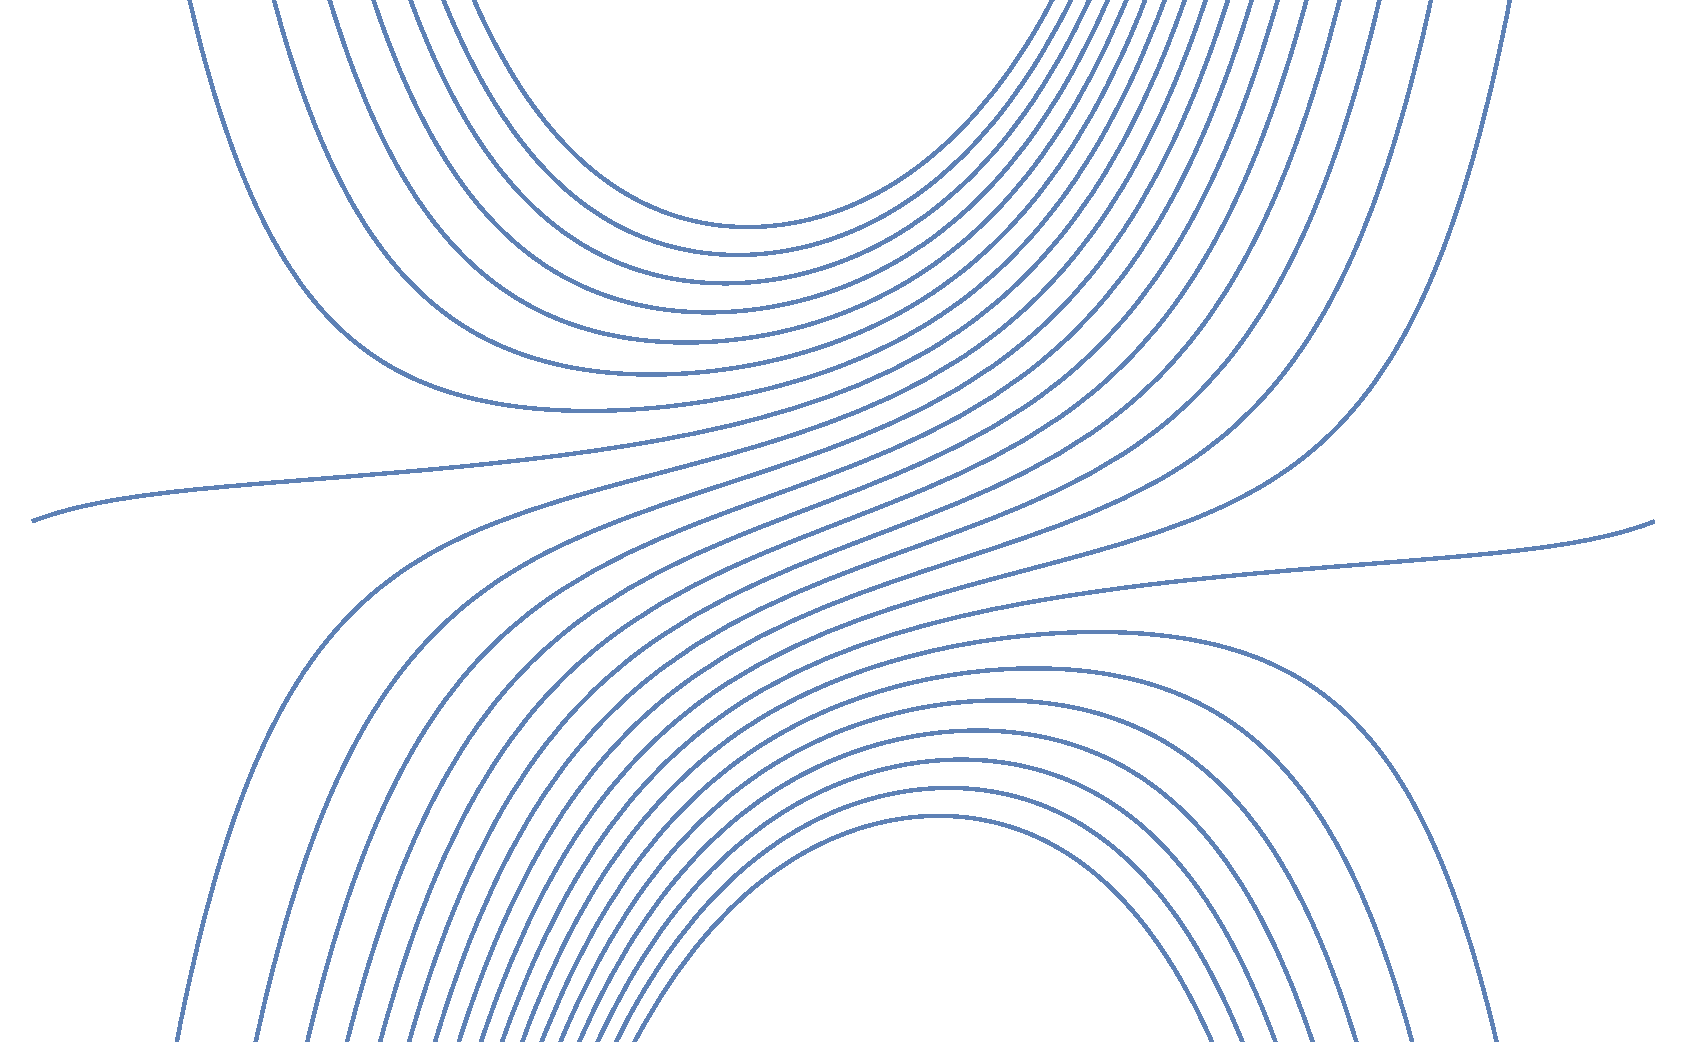
\includegraphics[scale=0.4]{../../Commun/Images/maths-cours-cauchy-1.pdf}};
\draw[->] (-6,0) -- (6,0) node[below] {$t$};
\draw[->] (0,-3.5) -- (0,3.5) node[left] {$y$};
\end{tikzpicture}
\end{center}
\remarque Le théorème de \nom{Cauchy-Lipschitz} prouve que la connaissance à l'instant $t_0$ d'un système régi par une équation différentielle résolue du premier ordre permet de connaitre complètement son passé et son futur.
\end{remarques}

\begin{exos}
\exo Résoudre sur $]0,+\infty[$ le problème de \nom{Cauchy}
  \[y(1)=1 \et y'(t)+\frac{y(t)}{t}=t.\]
Tracer le graphe de la solution.
\begin{sol}
Avec la variation de la constante, on trouve que les solutions de $(E)$ sont les $x\to t^2/3+c/t$ avec $c\in \R$. Et on trouve $c=2/3$ avec la condition initiale.
\end{sol}
\exo Montrer que les solutions de l'équation différentielle
  \[\forall t\in\R \qsep y'(t)+t\arctan(t^4+1)y(t)=\sh t\]
  sont toutes paires.
\end{exos}
\begin{sol}
Si $y$ est une solution sur $\R$, on définit $g$ par $g(t)=y(-t)$. On montre qu'alors $g$ est solution de $(E)$ sur $\R$. Or, $g(0)=y(0)$ donc $g$ et $y$ sont solutions du même pb de Cauchy. Elles sont donc égales.
\end{sol}

\subsection{Équation différentielle non résolue}

\begin{exoUnique}
\exo Résoudre l'équation différentielle
  $(t^2\ln t)y'(t)-ty(t)=-(1+\ln t)$ sur $\RPs$.
%Étant donnés $t_0\in\RPs$ et
%$y_0\in\R$, discuter le problème de Cauchy $y(t_0)=y_0$.
  \begin{sol}
  Sur chaque intervalle, on trouve $y(t)=1/t+c\ln t$ avec $c$ une constante différente. On raisonne par analyse-synthèse pour avoir une solution sur $\RPs$. L'existence de la dérivée impose aux deux constantes d'être égales. On le voit en écrivant l'égalité des limites des taux d'accroissements à gauche et à droite. Synthèse évidente. Les solutions sur $\RPs$
  sont $y(t)=1/t+c\ln t$.
  \end{sol}
%\exo Résoudre l'équation différentielle $t(t+1)y'+y=0$ sur
%  $\intero{-1}{+\infty}$.
%Étant donnés $t_0>-1$ et $y_0\in\R$, discuter le
%  problème de Cauchy $y(t_0)=y_0$.
\end{exoUnique}

\begin{remarqueUnique}
\remarque Pour les équations différentielles non résolues du premier ordre, 
  contrairement à ce qui se passe pour les équations résolues, il est possible
  qu'un problème de \nom{Cauchy} admette plusieurs solutions ou aucune. Voici par exemple
  plusieurs solutions au problème de \nom{Cauchy}
  \[y(1)=1, \et \forall t>0\qsep (t^2\ln t)y'(t)-ty(t)=-(1+\ln t).\]
\begin{center}
\begin{tikzpicture}[>=latex]
\node at (0,0) {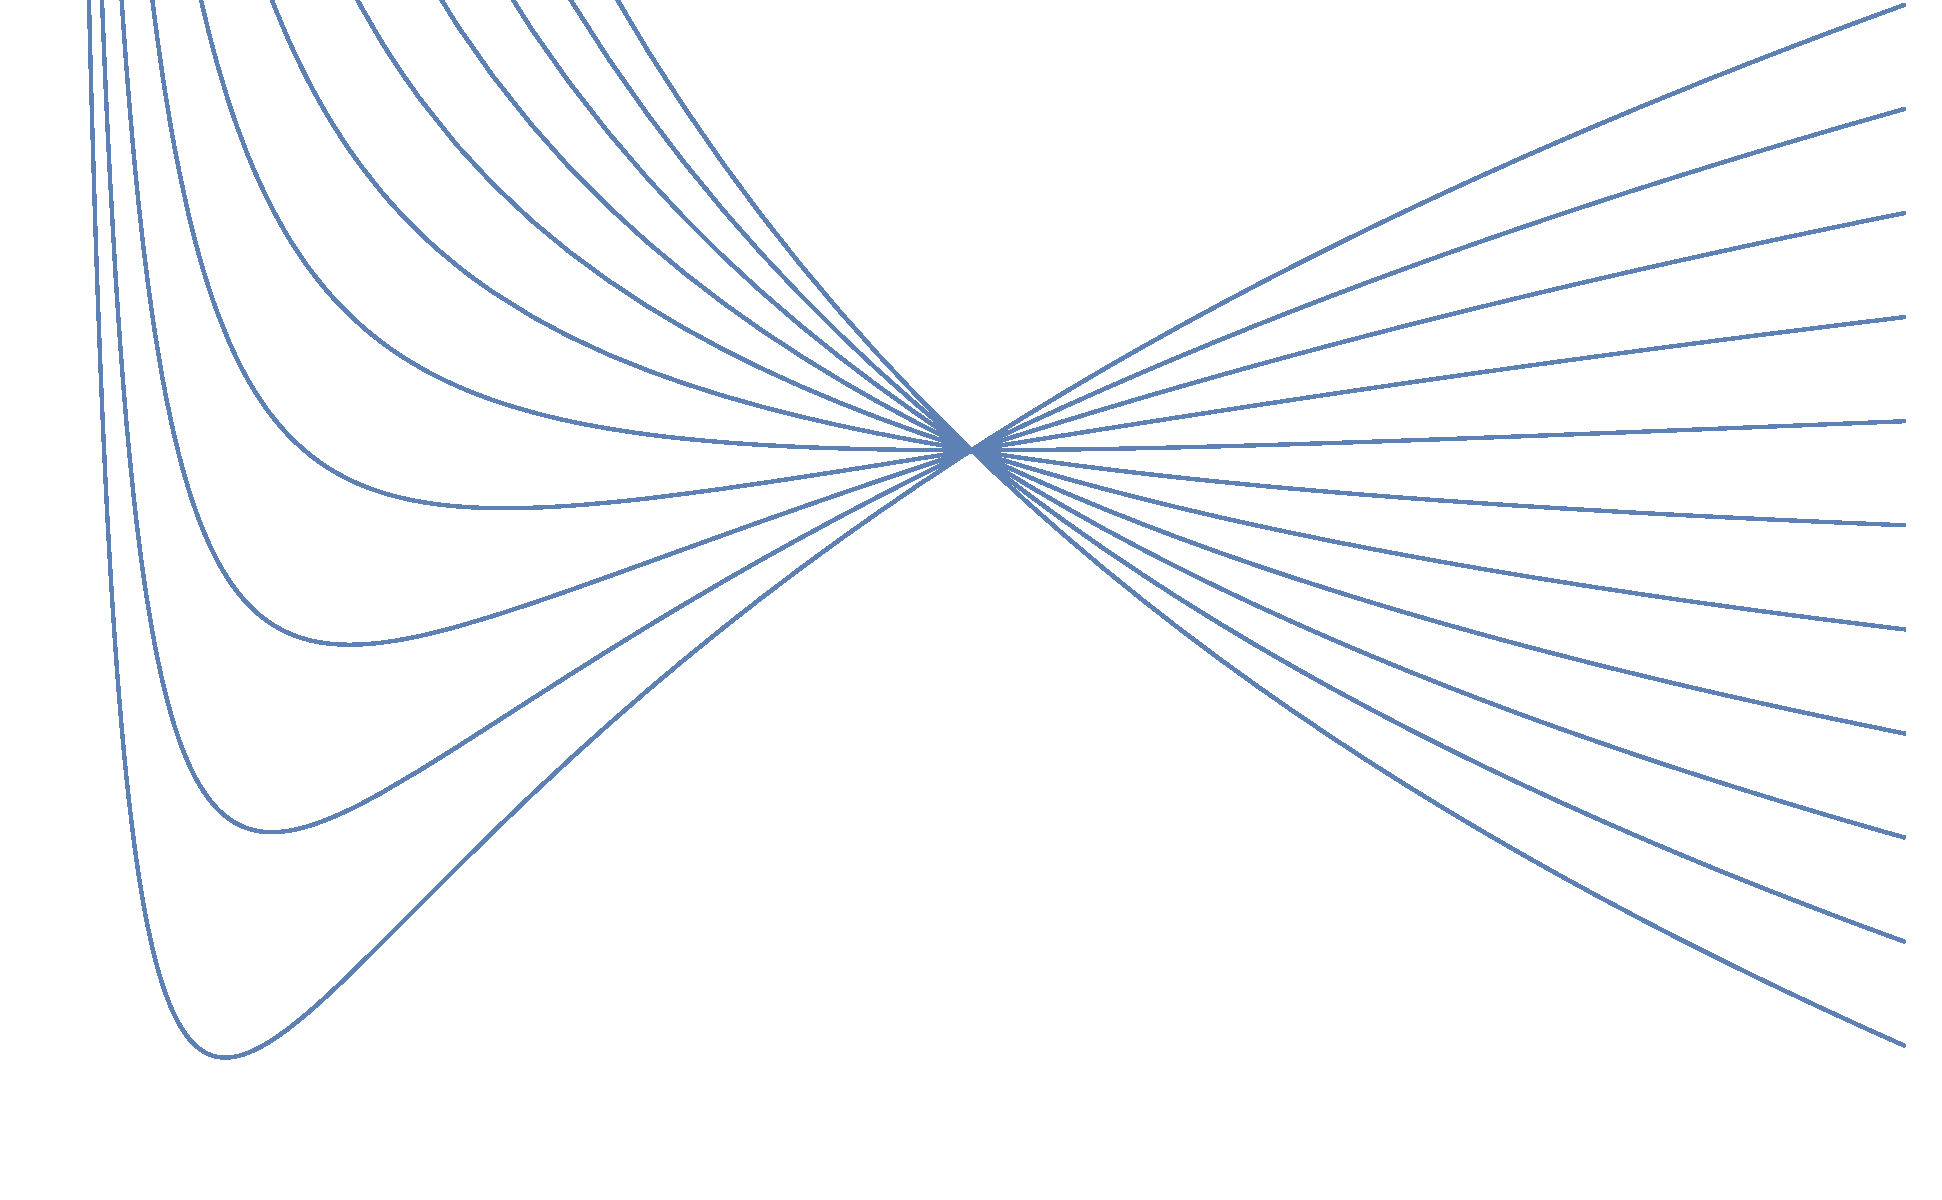
\includegraphics[scale=0.4]{../../Commun/Images/maths-cours-cauchy-3.pdf}};
\draw[->] (-6,0) -- (6.5,0) node[below] {$t$};
\draw[->] (-6,-4.2) -- (-6,4.2) node[left] {$y$};
\draw[shift={(0,0)}] (0pt,2pt) -- (0pt,-2pt) node[below] {1};
\draw[shift={(-6,1.1)}] (-2pt,0pt) -- (2pt,0pt) node[left] {1};
\end{tikzpicture}
\end{center}
  On peut aussi remarquer que pour $y_0\neq 1$, il n'existe aucune solution de cette équation différentielle
  vérifiant $y(1)=y_0$.
\end{remarqueUnique}

% \subsection{Méthode d'\nom{Euler}}

% On note $y$ la solution au problème de \nom{Cauchy}
% \[\begin{cases}
%   \forall t\in I \qsep y'(t)+a(t)y(t)=b(t)&\\
%   y(t_0)=y_0. &
%   \end{cases}\]
% Étant donnés $n\in\N$ et $\epsilon>0$ (supposé petit), la méthode d'Euler est
% une méthode permettant de calculer une valeur approchée
% de $u_n=y(t_0+n\epsilon)$. Comme $\epsilon$ est petit, l'approximation
% \[y'(t_0+n\epsilon)\approx
%   \frac{y(t_0+(n+1)\epsilon)-y(t_0+n\epsilon)}{\epsilon}=
%   \frac{u_{n+1}-u_n}{\epsilon}\]
% est raisonnable. $y$ étant solution de l'équation différentielle, on
% en déduit que
% \[y'(t_0+n\epsilon)+a(t_0+n\epsilon)y(t_0+n\epsilon)=b(t_0+n\epsilon)\]
% ce qui permet d'avoir une approximation de $u_{n+1}$ en fonction de $u_n$
% \[u_{n+1} \approx (1-\epsilon a(t_0+n\epsilon))u_n+\epsilon b(t_0+n\epsilon)\]
% Comme $u_0=y_0$, on calcule de proche en proche une valeur approchée de
% $u_n$.\\

% Par exemple, si $y$ est la solution au problème de \nom{Cauchy}
% \[\begin{cases}
%   \forall t\in \R \qsep y'(t)=y(t)&\\
%   y(0)=1 &
%   \end{cases}\]
% on sait que $y=\exp$.
% On se fixe $t>0$ et
% on souhaite calculer une valeur approchée de $y(t)$. Pour cela, on se donne
% $n\in\Ns$ et on pose $\epsilon=t/n$. On définit, pour tout $k\in\intere{0}{n}$,
% $u_k=y(k\epsilon)$. On a, d'après la méthode d'Euler
% \[u_0=1 \et \forall k\in\intere{0}{n-1} \qsep u_{k+1}\approx (1+\epsilon)u_k.\]
% Donc
% \[y(t)=u_n\approx (1+\epsilon)^n=\p{1+\frac{t}{n}}^n.\]
% On vérifie que lorsque $n$ tend vers $+\infty$, $(1+t/n)^n$ tend vers $\e^t$.
% Sur cet exemple, lorsque le pas $\epsilon$ tend vers $0$, la valeur approchée de
% $y(t)$, calculée par la méthode d'Euler, tend bien vers la valeur exacte de
% $y(t)$.

\section{Équation différentielle linéaire du second ordre}

\begin{definition}
Soit $a,b,c,d:I\to\K$ des fonctions définies sur un intervalle $I$. On appelle solution sur $I$ de l'équation différentielle linéaire du second ordre $ay''+by'+cy=d$, toute fonction $y:I\to\K$, dérivable deux fois sur $I$, telle que
\[\forall t\in I \qsep a(t)y''(t)+b(t)y'(t)+c(t)y(t)=d(t).\]
On dit que l'équation est \emph{résolue} lorsque $a$ ne s'annule pas et qu'elle est \emph{homogène} lorsque la fonction $d$ est nulle.
\end{definition}

\subsection{Équation différentielle homogène}

\begin{proposition}[utile=-3]
Soit $a,b,c\in\C$ avec $a\neq 0$ et $(E)$ l'équation différentielle
\[\forall t\in\R \qsep a y''(t)+by'(t)+cy(t)=0.\]
On résout sur $\C$ l'équation caractéristique $az^2+bz+c=0$.
\begin{itemize}
\item Si cette équation possède deux racines distinctes $r_1$ et $r_2$
  ($\Delta\neq 0$), alors les solutions complexes de $(E)$ sont les fonctions
  \[\dspappli{y_{\lambda,\mu}}{\R}{\C}{t}{\lambda \e^{r_1 t}+\mu \e^{r_2 t}}\]
  où $\lambda,\mu\in\C$.
\item Si cette équation admet une racine double $r$ ($\Delta=0$), alors les
  solutions complexes de $(E)$ sont les fonctions
  \[\dspappli{y_{\lambda,\mu}}{\R}{\C}{t}{\p{\lambda t+\mu}\e^{r t}}\]
  où $\lambda,\mu\in\C$.
\end{itemize}
\end{proposition}

\begin{preuve}
\begin{francois}
Soit $a, b, c\in\C$ avec $a\neq 0$. On considère l'équation différentielle
\[(E)\qquad \forall t\in\R \qsep a y''(t)+by'(t)+cy(t)=0.\]
On commence par chercher les solutions de $(E)$ qui sont de la forme $t\mapsto\e^{r t}$. Soit $r\in\C$ et $y$ la fonction de $\R$ dans $\C$ définie par
\[\forall t\in\R\qsep y(t)\defeq\e^{rt}.\]
D'après les théorèmes usuels, $y$ est dérivable deux fois sur $\R$ et
\begin{eqnarray*}
\forall t\in\R\qsep y'(t)&=&r\e^{rt}\\
y''(t)&=&r^2\e^{rt}.
\end{eqnarray*}
Donc
\begin{eqnarray*}
\text{$y$ est solution de $(E)$}
&\ssi& \forall t\in\R \qsep a y''(t)+by'(t)+cy(t)=0\\
&\ssi& \forall t\in \R\qsep (ar^2+br+c)\e^{rt}=0\\
&\ssi& ar^2+br+c=0.
\end{eqnarray*}
Puisqu'on est sur $\C$, cette équation $(E_c)$ admet au moins une solution $r_1\in\C$. La fonction $t\mapsto \e^{r_1 t}$ est donc une solution de $(E)$. Pour trouver l'ensemble des solutions de $(E)$, on va appliquer la méthode de la variation de la constante. Soit $y$ une fonction dérivable deux fois sur $\R$. On définit la fonction $u$ sur $\R$ par
\[\forall t\in\R\qsep u(t)\defeq y(t)\e^{-r_1 t}.\]
D'après les théorèmes usuels, $u$ est dérivable deux fois sur $\R$. De plus
\begin{eqnarray*}
\forall t\in\R\qsep y(t)&=&u(t)\e^{r_1 t}\\
y'(t)&=&\cro{u'(t)+r_1 u(t)}\e^{r_1 t}\\
y''(t)&=&\cro{u''(t)+2r_1 u'(t)+r_1^2 u(t)}\e^{r_1 t}.
\end{eqnarray*}
On en déduit que
\begin{eqnarray*}
\text{$y$ est solution de $(E)$}
&\ssi& \forall t\in\R \qsep a y''(t)+by'(t)+cy(t)=0\\
&\ssi& \forall t\in \R\qsep \cro{a u''(t)+\p{2ar_1+b}u'(t)+(ar_1^2+br_1+c)u(t)}\e^{r_1 t}=0\\
&\ssi& \forall t\in \R\qsep a u''(t)+\p{2ar_1+b}u'(t)+\underbrace{(ar_1^2+br_1+c)}_{=0}u(t)=0\\
&\ssi& \forall t\in \R\qsep a u''(t)+\p{2ar_1+b}u'(t)=0\\
&\ssi& \forall t\in \R\qsep u''(t)+\p{2r_1+\frac{b}{a}}u'(t)=0.
\end{eqnarray*}
On remarque que $y$ est une solution de $(E)$ si et seulement si $u'$ est solution d'une équation différentielle linéaire d'ordre 1 que l'on sait résoudre. La méthode de la variation de la constante nous a donc permis de faire baisser l'ordre de l'équation différentielle.
\begin{itemize}
\item Si l'équation caractéristique $(E_c)$ admet deux racines distinctes $r_1$ et $r_2$. Alors, les relations coefficients racines, donnent
\[r_1+r_2=-\frac{b}{a}\]
donc
\begin{eqnarray*}
\text{$y$ est solution de $(E)$}
&\ssi& \forall t\in \R\qsep u''(t)+\p{r_1-r_2}u'(t)=0\\
&\ssi& \forall t\in \R\qsep u''(t)\e^{(r_1-r_2)t}+\p{r_1-r_2}u'(t)\e^{(r_1-r_2)t}=0\\
&\ssi& \forall t\in\R\qsep \frac{{\rm d}}{{\rm d}t}\p{u'(t)\e^{(r_1-r_2)t}}=0\\
&\ssi& \exists\lambda\in\C\qsep \forall t\in\R\qsep u'(t)\e^{(r_1-r_2)t}=\lambda\\
&\ssi& \exists\lambda\in\C\qsep \forall t\in\R\qsep u'(t)=\lambda \e^{(r_2-r_1)t}\\
&\ssi& \exists\lambda,\mu\in\C\qsep \forall t\in\R\qsep u(t)=\frac{\lambda}{r_2-r_1} \e^{(r_2-r_1)t}+\mu\\
&\ssi& \exists\lambda,\mu\in\C\qsep \forall t\in\R\qsep u(t)=\mu+\lambda \e^{(r_2-r_1)t}\\
&\ssi& \exists\lambda,\mu\in\C\qsep \forall t\in\R\qsep y(t)\e^{-r_1 t}=\mu+\lambda \e^{(r_2-r_1)t}\\
&\ssi& \exists\lambda,\mu\in\C\qsep \forall t\in\R\qsep y(t)=\mu \e^{r_1 t}+\lambda \e^{r_2 t }.
\end{eqnarray*}
Les solutions de $(E)$ sont donc les fonctions
\[\dspappli{y_{\lambda,\mu}}{\R}{\C}{t}{\lambda \e^{r_1 t}+\mu \e^{r_2 t}}\]
où $\lambda,\mu\in\C$.
\item Si l'équation caractéristique $(E_c)$ admet une unique racine, les relations coefficients racines donnent
\[2r_1=-\frac{b}{a}\]
donc
\begin{eqnarray*}
\text{$y$ est solution de $(E)$}
&\ssi& \forall t\in \R\qsep u''(t)=0\\
&\ssi& \exists\lambda\in\C\qsep \forall t\in \R\qsep u'(t)=\lambda\\
&\ssi& \exists\lambda,\mu\in\C\qsep \forall t\in \R\qsep u(t)=\lambda t+\mu\\
&\ssi& \exists\lambda,\mu\in\C\qsep \forall t\in\R\qsep y(t)\e^{-r_1 t}=\lambda t+\mu\\
&\ssi& \exists\lambda,\mu\in\C\qsep \forall t\in\R\qsep y(t)=(\lambda t+\mu) \e^{r_1 t}
\end{eqnarray*}
Les solutions de $(E)$ sont donc les fonctions
\[\dspappli{y_{\lambda,\mu}}{\R}{\C}{t}{(\lambda t+\mu)\e^{r_1 t}}\]
où $\lambda,\mu\in\C$.
\end{itemize}
\end{francois}
\begin{victor}
\begin{itemize}
\item [$\bullet$] Cherchons d'abord des solutions exponentielles de $(E)$. Soit $r\in \C$. Définissons $\dspappli{u}{\R}{\C}{t}{\e^{rt}}$.
\begin{eqnarray*}
u \in \mathcal{S}(E) &\Longleftrightarrow& \forall t\in \R, (ar^2+br+c)\e^{rt}=0\\
&\Longleftrightarrow& \forall x\in \R, (ar^2+br+c)=0
\end{eqnarray*}
\item [$\bullet$] \underline{Méthode de l'abaissement de l'ordre :}

Supposons que l'on dispose de $r\in\C$ une racine de $(EC)$. \underline{Principe de la méthode :} chercher des solutions de $(E)$ sous la forme $x\mapsto \e^{rt}v(t)$.

Soit $u:\R\to \K$ deux fois dérivables. Définissons $\dspappli{v}{\R}{\C}{t}{\e^{-rt}u(t)}$. $v$ est deux fois dérivables sur $\R$ et $\forall x\in\R$ :
\[u'(t)=\p{rv(t)+v'(t)}\e^{rt}\]
\[u''(t)=\p{v''(t)+2rv'(t)+r^2v(t)}\e^{rt}\]

Ainsi,
\begin{eqnarray*}
u\in \mathcal{S}(E)&\Longleftrightarrow & \forall t\in \R, au''(t)+bu'(t)+cu(t)=0\\
&\Longleftrightarrow & \forall t\in \R, v''(t)\p{a\e^{rt}}+v'(t)\p{2ar\e^{rt}+b\e^{rt}}+v(t)\p{ar^2\e^{rt}+br\e^{rt}+c\e^{rt}}=0\\
&\Longleftrightarrow & \forall t\in \R, av''(t)+\p{2ar+b}v'(t)+\p{ar^2+br+c}v(t)=0\\
&\Longleftrightarrow & \forall t\in \R, av''(t)+\p{2ar+b}v'(t)=0\\
&\Longleftrightarrow & v' \text{ est solution de } (E') : y'+\p{2r+\dfrac{b}{a}}y=0
\end{eqnarray*}
La solution générale de $(E')$ est : $t\mapsto \lambda \e^{-\p{2r+\dfrac{b}{a}}t}$. On est alors amené à distinguer deux cas pour la primitive :

\item [$\bullet$] \underline{Premier cas : } $2r+\dfrac{b}{a}=0$, i.e $r=\dfrac{-b}{2a}$. \textbf{C'est le cas où le discriminant de l'EC est nul.}
\begin{eqnarray*}
u\in \mathcal{S}(E)&\Longleftrightarrow & \exists \lambda\in\K \text{ tel que } \forall t \in \R, v'(t)=\lambda\\
&\Longleftrightarrow & \exists (\lambda,\mu)\in\K^2 \text{ tel que } \forall t \in \R, v(t)=\lambda t+\mu\\
&\Longleftrightarrow & \exists (\lambda,\mu)\in\K^2 \text{ tel que } \forall t \in \R, u(t)=(\lambda t+\mu)\e^{rt}
\end{eqnarray*}

\item [$\bullet$] \underline{Deuxième cas : } Lorsque le discriminant de l'EC est non nul. Notons $r'$ la seconde racine de l'EC. Alors, par exemple, avec $\delta$ une racine du discriminant dans $\C$ :
\[r=\dfrac{-b+\delta}{2a} \quad ; \quad r'=\dfrac{-b-\delta}{2a}\]
Ainsi, $-\p{2r+\dfrac{b}{a}}=r'-r$. D'où :
\begin{eqnarray*}
u\in \mathcal{S}(E)&\Longleftrightarrow & \exists \lambda\in\K \text{ tel que } \forall t \in \R, v'(t)=\lambda\e^{(r'-r)t}\\
&\Longleftrightarrow & \exists (\lambda,\mu)\in\K^2 \text{ tel que } \forall t \in \R, v(t)=\frac{\lambda}{r'-r}\e^{(r'-r)t}+\mu\\
&\Longleftrightarrow & \exists (\lambda,\mu)\in\K^2 \text{ tel que } \forall t \in \R, u(t)=\frac{\lambda}{r'-r}\e^{r't}+\mu\e^{rt}\\
&\Longleftrightarrow & \exists (\lambda,\mu)\in\K^2 \text{ tel que } \forall t \in \R, u(t)=\lambda\e^{r't}+\mu\e^{rt} \text{ quitte à changer }\lambda.
\end{eqnarray*}
\end{itemize}
\end{victor}
\end{preuve}

% \begin{remarques}
% \remarque L'ensemble des solutions complexes de cette équation différentielle
%   est un \Cev de dimension 2.
% \end{remarques}

\begin{exoUnique}
\exo Résoudre l'équation différentielle $y''-3y'+2y=0$.
\end{exoUnique}

\begin{proposition}[utile=-3]
Soit $a,b,c\in\R$ avec $a\neq 0$ et $(E)$ l'équation différentielle
\[\forall t\in\R \qsep a y''(t)+by'(t)+cy(t)=0.\]
On résout sur $\C$ l'équation caractéristique $az^2+bz+c=0$.
\begin{itemize}
\item Si cette équation possède deux racines réelles distinctes $r_1$ et $r_2$
  ($\Delta> 0$), alors les solutions réelles de $(E)$ sont les fonctions
  \[\dspappli{y_{\lambda,\mu}}{\R}{\R}{t}{\lambda \e^{r_1 t}+\mu \e^{r_2 t}}\]
  où $\lambda,\mu\in\R$.
\item Si cette équation admet une racine double $r$ ($\Delta=0$), alors les
  solutions réelles de $(E)$ sont les fonctions
  \[\dspappli{y_{\lambda,\mu}}{\R}{\R}{t}{\p{\lambda t+\mu}\e^{r t}}\]
  où $\lambda,\mu\in\R$.
\item Si cette équation admet deux racines complexes conjuguées $r+\ii\omega$ et
  $r-\ii\omega$ ($\Delta <0$), alors les solutions réelles de $(E)$ sont les
  fonctions
  \[\dspappli{y_{\lambda,\mu}}{\R}{\R}{t}{\cro{\lambda\cos\p{\omega t}+
    \mu\sin\p{\omega t}}\e^{r t}}\]
  où $\lambda,\mu\in\R$.
\end{itemize}
\end{proposition}

\begin{preuve}
\begin{francois}
Soit $a,b,c\in\R$ avec $a\neq 0$. On considère l'équation différentielle
\[(E)\qquad\forall t\in\R \qsep a y''(t)+by'(t)+cy(t)=0\]
ainsi que son équation caractéristique associée $(E_c)$~: $az^2+bz+c=0$.
\begin{itemize}
\item Si $\Delta>0$ ou $\Delta=0$, l'équation caractéristique admet au moins une solution réelle $r_1$. La démonstration faite dans le cas de la recherche des solutions complexes s'adapte simplement et permet de trouver l'ensemble des solutions réelles de $(E)$.
\item Si $\Delta<0$, l'équation caractéristique admet deux solutions complexes conjuguées $r+\ii\omega$ et $r-\ii\omega$. Montrons que les solutions réelles de $(E)$ sont les fonctions
\[t\mapsto \cro{\lambda\cos\p{\omega t}+\mu\sin\p{\omega t}}\e^{r t}\]
où $\lambda,\mu\in\R$.
\begin{itemize}
\item Ce sont des solutions de $(E)$. En effet, soit $\lambda,\mu\in\R$ et $y$ la fonction définie sur $\R$ par
\[\forall t\in\R\qsep y(t)\defeq \cro{\lambda\cos\p{\omega t}+\mu\sin\p{\omega t}}\e^{r t}.\]
Alors
\begin{eqnarray*}
\forall t\in\R\qsep y(t)
&=& \cro{\lambda\cos\p{\omega t}+\mu\sin\p{\omega t}}\e^{r t}\\
&=& \cro{\lambda\frac{\e^{\ii\omega t}+\e^{-\ii\omega t}}{2}+\mu\frac{\e^{\ii\omega t}-\e^{-\ii\omega t}}{2\ii}}\e^{r t}\\
&=& \underbrace{\p{\frac{\lambda}{2}+\frac{\mu}{2\ii}}}_{\eqdef \alpha\in\C}\e^{(r+\ii\omega)t}+\underbrace{\p{\frac{\lambda}{2}-\frac{\mu}{2\ii}}}_{\eqdef \beta\in\C}\e^{(r-\ii\omega)t}.
\end{eqnarray*}
D'après la proposition précédente, on en déduit que $y$ est une solution de $(E)$.
\item Ce sont les seules solutions réelles de $(E)$. En effet, soit $y$ une solution réelle de $(E)$. Alors, c'est une solution complexe, donc d'après la proposition précédente, il existe $\lambda,\mu\in\C$ tels que
\[\forall t\in\R\qsep y(t)=\lambda\e^{(r+\ii\omega)t}+\mu\e^{(r-\ii\omega)t}.\]
Il existe $\alpha,\beta,\gamma,\delta\in\R$ tels que $\lambda=\alpha+\ii\beta$ et $\mu=\gamma-\ii\delta$. Alors
\begin{eqnarray*}
\forall t\in\R\qsep y(t)
&=& \Re\cro{y(t)}\quad\text{car $y$ est réelle}\\
&=& \Re\cro{\p{\alpha+\ii\beta}\e^{(r+\ii\omega)t}+\p{\gamma+\ii\delta}\e^{(r-\ii\omega)t}}\\
&=& \Re\cro{\p{\alpha+\ii\beta}\p{\cos(\omega t)+\ii\sin(\omega t)}+\p{\gamma+\ii\delta}\p{\cos(\omega t)-\ii\sin(\omega t)}}\e^{rt}\\
&=& [\underbrace{(\alpha+\gamma)}_{\eqdef \lambda'\in\R}\cos(\omega t)+\underbrace{(\gamma-\beta)}_{\eqdef \mu'\in\R}\sin(\omega t)]\e^{rt}
\end{eqnarray*}
donc $y$ est bien de la forme demandée.
\end{itemize}
\end{itemize}
\end{francois}
\begin{victor}
Les deux premiers cas sont une conséquence de la proposition précédente. Il reste donc à traiter le cas où $\Delta<0$.

L'EC admet alors deux racines $r\pm i\omega$. 

\underline{Analyse :} Soit $y:\R\to\R$ une solution de $(E)$. D'après la proposition précédente, on peut fixer $(A,B)\in \C^2$ tels que \[\forall t\in\R, y(t)=A\e^{(r+i\omega)t}+B\e^{(r-i\omega)t}=\e^{rt}\p{A\e^{i\omega t}+B\e^{-i\omega t}}.\]
Or, $\forall t\in\R, y(t)=\Re(y(t))=\e^{rt}\Re\p{A\e^{i\omega t}+B\e^{-i\omega t}}$ qui est donc de la forme $y(t)=\cro{c_1\cos\p{\omega t}+c_2\sin\p{\omega t}}\e^{r t}$.

\underline{Synthèse :} Réciproquement, soit $(c_1,c_2)\in\R^2$. Définissons $\dspappli{y}{\R}{\R}{t}{\cro{c_1\cos\p{\omega t}+c_2\sin\p{\omega t}}\e^{r t}}$.
On applique les formules d'Euler pour s'apercevoir que $y$ ainsi définie est bien solution de $(E)$ car de la forme des solutions de la proposition précédente.
\end{victor}
\end{preuve}

\begin{remarqueUnique}
% \remarque L'ensemble des solutions réelles de cette équation différentielle
%   est un \Rev de dimension 2.
\remarque Dans le cas où l'équation caractéristique admet deux racines complexes
  conjuguées, les solutions de $(E)$ peuvent s'écrire sous la forme
  \[\dspappli{y_{\lambda,\phi}}{\R}{\R}{t}{\lambda \sin\p{\omega t-\phi}\e^{r t}}\]
  où $\lambda,\phi\in\R$. Lors de la recherche effective de tels coefficients, 
  quitte à changer $\phi$ en $\phi+\pi$, on impose souvent $\lambda\in\RP$.
% \remarque Étant donnés $t_0\in\R$ et $y_0,y_1\in\R$, on appelle problème de
%   \nom{Cauchy} la recherche des solutions $y$ de l'équation différentielle
%   $ay''+by'+cy=0$ telles que $y(t_0)=y_0$ et $y'(t_0)=y_1$. On peut montrer
%   que tout problème de \nom{Cauchy} admet une et une seule solution.
\end{remarqueUnique}

\begin{exos}
\exo Résoudre l'équation différentielle $y''+2y'+2y=0$.
\exo Soit $\omega_0\in\R$. Résoudre l'équation différentielle
  $y''+\omega_0^2 y=0$.
\exo En effectuant le changement de fonction inconnue $z(t)= t^2 y(t)$,
  résoudre l'équation différentielle
  \[\forall t\in\RPs \qsep t^2 y''(t)+4ty'(t)+(2-t^2)y(t)=0.\]
  \begin{sol}
  On trouve $z''-z=0$. Donc $y(t)=(ae^t+be^{-t})/t^2$.
  \end{sol}
\exo En effectuant le changement de variable $t=\sqrt{u}$, résoudre
  l'équation différentielle
  \[\forall t\in\RPs \qsep ty''(t)-y'(t)+4t^3y(t)=0.\]
  \begin{sol}
  On définit la fonction $z$ sur $\RPs$ par $z(u)=y(\sqrt{u})$, donc
  $y(t)=z(t^2)$. L'équation devient alors $z''+z=0$. Les solutions sont donc
  les $y(t)=c_1\cos(t^2)+c_2\sin(t^2)$.
  \end{sol}
\end{exos}

\subsection{Équation différentielle avec second membre}

\begin{proposition}[utile=-3,nom={Théorème de superposition}]
Soit $a,b,c,d:I\to\K$ des fonctions définies sur un intervalle $I$.
Si $y_p$ est une solution \og particulière \fg de l'équation différentielle
\[\forall t\in\R \qsep a(t)y''(t)+b(t)y'(t)+c(t)y(t)=d(t)\]
alors les solutions de cette équation différentielle sont les fonctions $y_p+y$
où $y$ parcourt l'ensemble des solutions de l'équation différentielle homogène
associée
\[\forall t\in\R \qsep a(t)y''(t)+b(t)y'(t)+c(t)y(t)=0.\]
\end{proposition}


\begin{proposition}[utile=-3,nom={Théorème de superposition}]
\begin{itemize}
\item Soit $a,b,c,d_1,d_2:I\to\K$ des fonctions définies sur un intervalle $I$, $\lambda,\mu\in\K$ et $y_{p_1},y_{p_2}:I\to\K$ des solutions \og particulières \fg des équations
  différentielles respectives $ay''+by'+cy=d_1$ et $ay''+by'+cy=d_2$. Alors
  $\lambda y_{p_1}+\mu y_{p_2}$ est une solution \og particulière \fg de l'équation différentielle
  \[\forall t\in\R \qsep a(t)y''(t)+b(t)y'(t)+c(t)y(t)=
    \lambda d_1(t)+\mu d_2(t).\]
\item Soit $a,b,c:I\to\R$ et $d:I\to\C$ des fonctions définies sur un intervalle $I$ et $y_p:I\to\C$ une solution
  \og particulière \fg de l'équation différentielle $ay''+by'+cy=d$. Alors
  $\Re(y_p)$ est une solution \og particulière \fg de l'équation différentielle
  \[\forall t\in \R \qsep a(t)y''(t)+b(t)y'(t)+c(t)y(t)=\Re(d(t)).\]
\end{itemize}
\end{proposition}

\begin{remarqueUnique}
\remarque Bien entendu, une proposition similaire existe pour la partie imaginaire.
\end{remarqueUnique}

\begin{proposition}[utile=-3]
Soit $a,b,c\in\C$ avec $a\neq 0$. Si $P$ est un polynôme de degré $n$ et
$\alpha\in\C$, alors l'équation différentielle
\[\forall t\in \R \qsep ay''(t)+by'(t)+cy(t)=P(t)\e^{\alpha t}\]
admet comme solution une (unique) fonction du type
$t\mapsto t^m Q(t)\e^{\alpha t}$ où $Q$ est un polynôme de degré $n$ et
$m$ est l'ordre de $\alpha$ comme racine de l'équation
caractéristique (avec par convention $m=0$ si $\alpha$ n'est pas racine
de cette équation).
\end{proposition}

\begin{exos}
\exo Déterminer les solutions de l'équation différentielle
  $y''(t)+y'(t)+y(t)=t^2$.
  \begin{sol}
  Les solutions sont les
  \[y(x)=\p{c_1\sin\p{\frac{\sqrt{3}}{2}c}+c_2\cos\p{\frac{\sqrt{3}}{2}c}}
    e^{-\frac{x}{2}}+x^2-2x\]
  \end{sol}
\exo Déterminer les solutions de l'équation différentielle
  $y''(t)+y(t)=t\cos t$.
  \begin{sol}
  On trouve
  \[\frac{1}{4}(-it^2+t)e^{it}\]
  puis
  \[\frac{1}{4}\p{t\cos t+t^2\sin t}\]
  \end{sol}
\end{exos}

\subsection{Problème de \nom{Cauchy}}

\begin{definition}[nom={Problème de \nom{Cauchy}}]
Soit $a,b,c,d:I\to\K$ des fonctions définies sur un intervalle $I$, $t_0\in I$ et
$y_0,y_1\in\K$. On appelle \emph{problème de \nom{Cauchy}} la recherche des solutions $y$ de
l'équation différentielle du second ordre
\[\forall t\in I \qsep a(t)y''(t)+b(t)y'(t)+c(t)y(t)=d(t)\]
telles que $y(t_0)=y_0$ et $y'(t_0)=y_1$.
\end{definition}

\begin{theoreme}[nom={Théorème de \nom{Cauchy-Lipschitz}}]
Soit $a,b,c:I\to\K$ des fonctions continues sur un intervalle $I$,
$t_0\in I$ et $y_0,y_1\in\K$. Alors il existe une et une seule solution à
l'équation différentielle résolue du second ordre
\[\forall t\in I \qsep y''(t)+a(t)y'(t)+b(t)y(t)=c(t)\]
telle que $y(t_0)=y_0$ et $y'(t_0)=y_1$.
\end{theoreme}

\begin{remarques}
\remarque Graphiquement, cette proposition signifie que par tout
  point $(t_0,y_0)\in I\times \R$ passe un et un seul graphe de pente $y_1\in\R$,
  solution de l'équation différentielle $y''(t)+a(t)y'(t)+b(t)y(t)=c(t)$. Les courbes intégrales peuvent se croiser, mais doivent avoir des pentes différentes lorsqu'elles se croisent. Par exemple, voici quelques
  solutions de l'équation différentielle
  \[\forall t\in\R\qsep y''(t)+y(t)=\frac{1}{2}t^2+t.\]
\begin{center}
\begin{tikzpicture}[>=latex]
\node at (0,0) {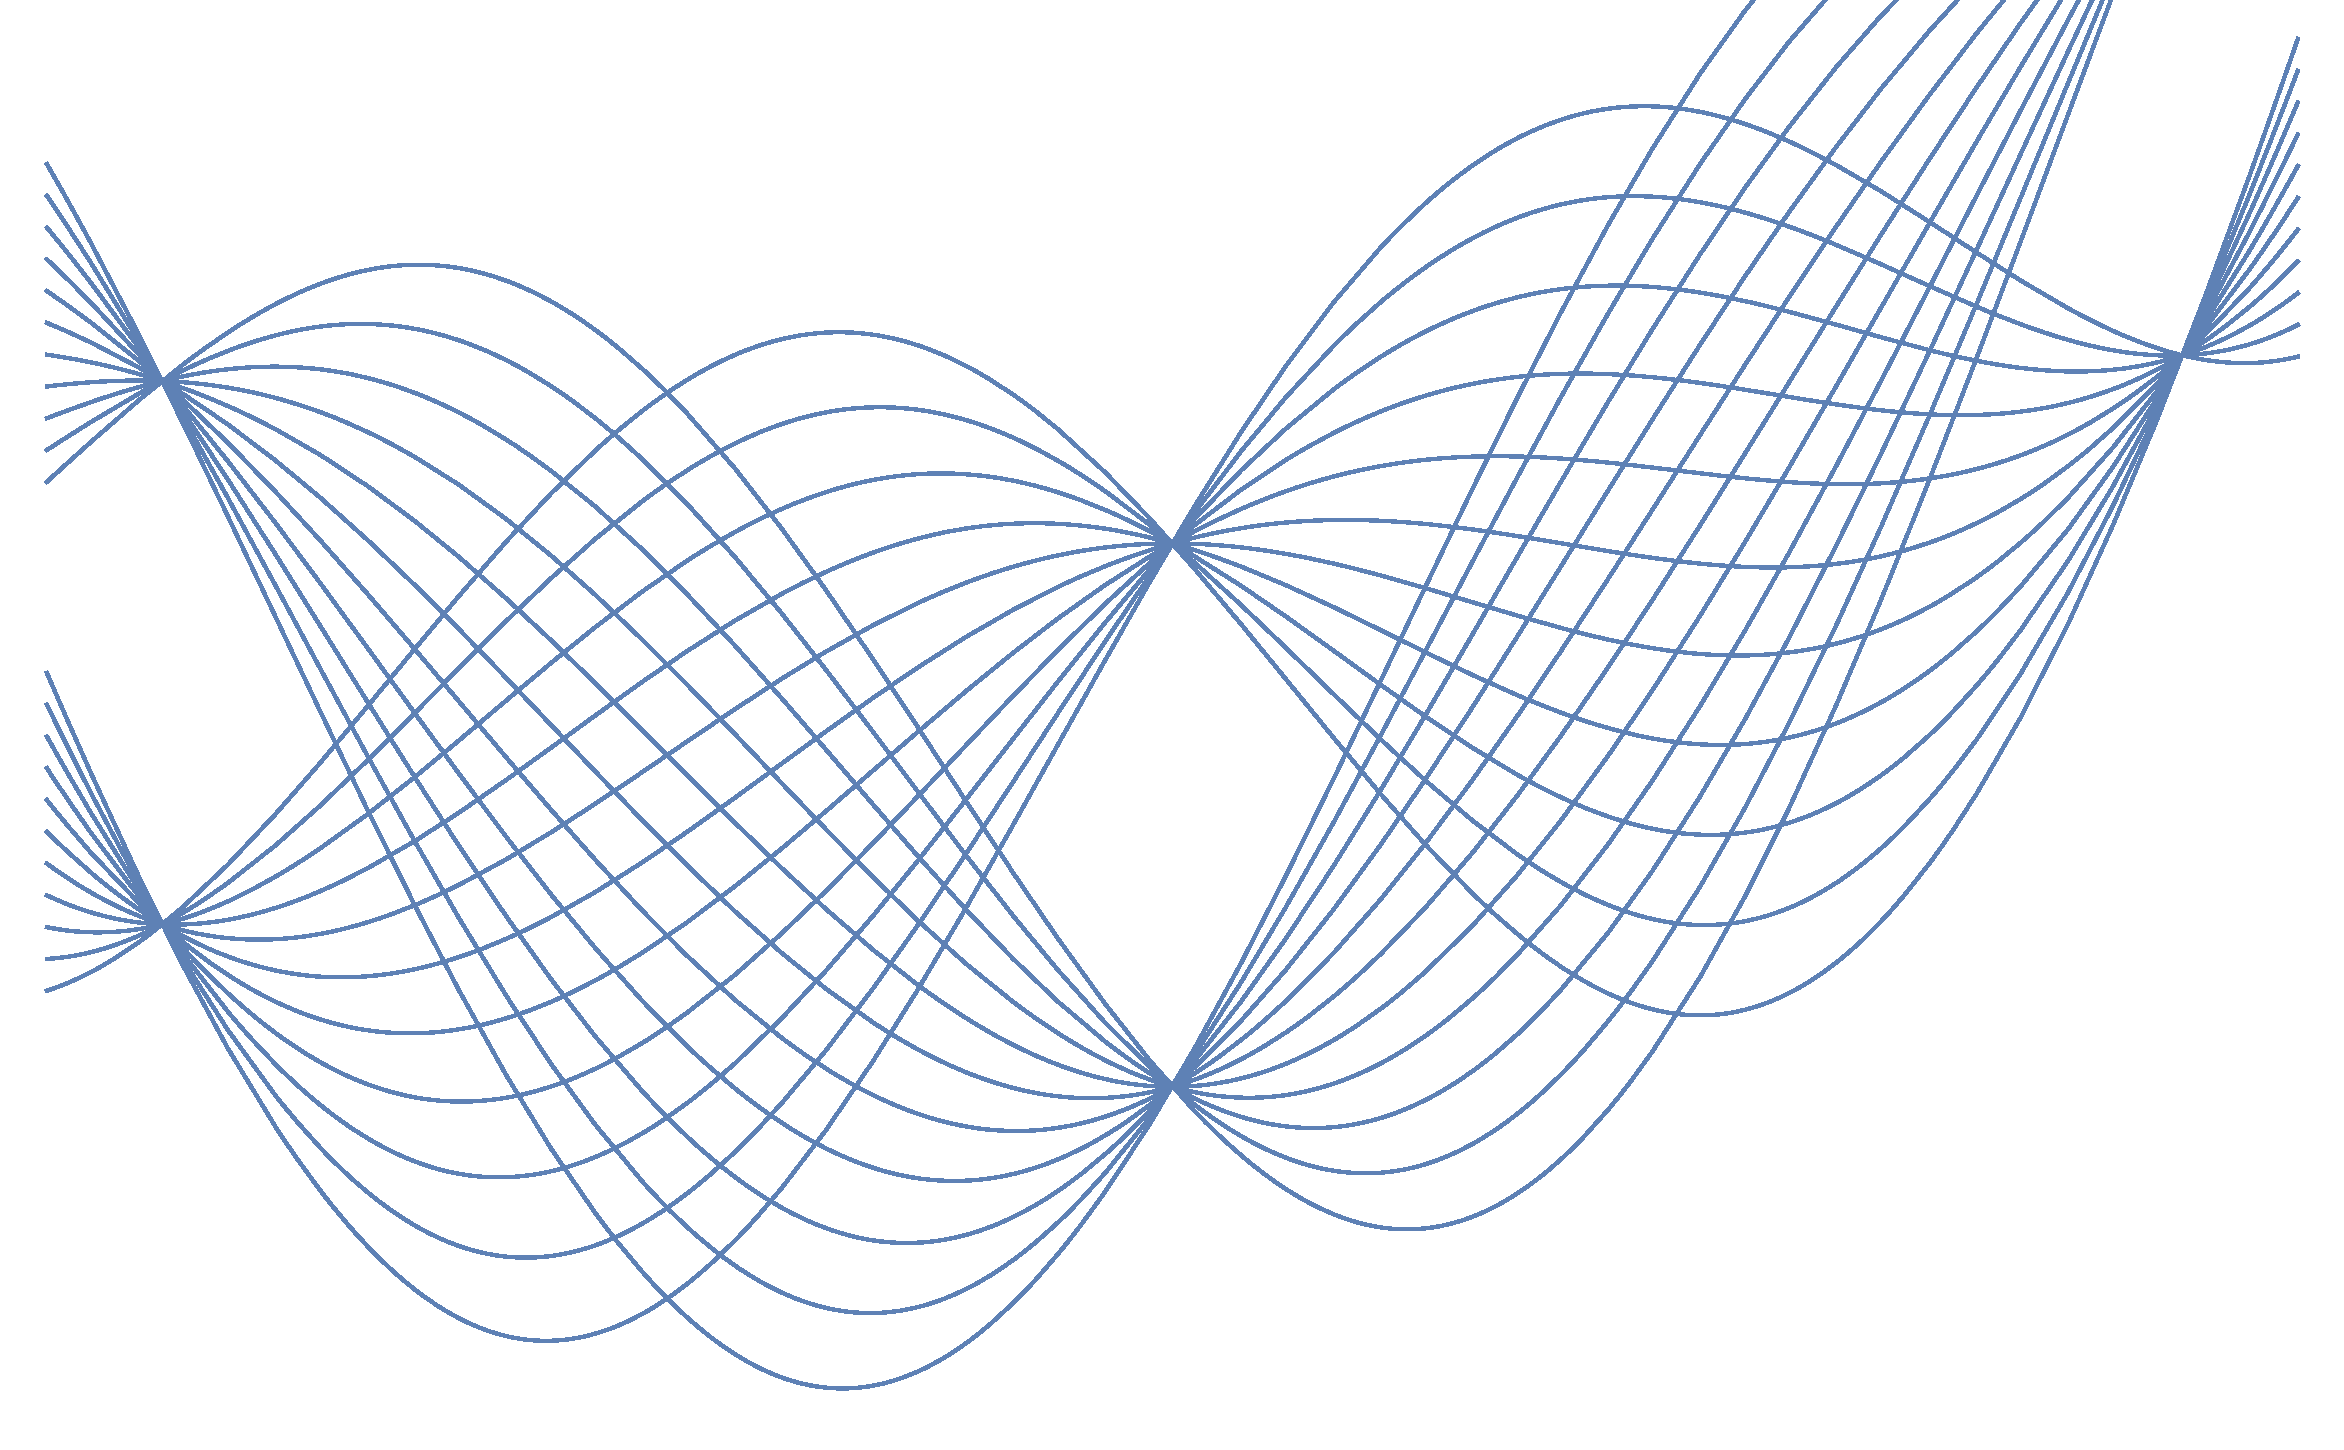
\includegraphics[scale=0.4]{../../Commun/Images/maths-cours-cauchy-2.pdf}};
\draw[->] (-7.65,0) -- (7.65,0) node[below] {$t$};
\draw[->] (0,-5) -- (0,5) node[left] {$y$};
\end{tikzpicture}
\end{center}
\remarque Le théorème de \nom{Cauchy-Lipschitz} prouve que la connaissance de la valeur de $y$ et de sa dérivée à l'instant $t_0$ d'un système régi par une équation différentielle résolue du second ordre permet de connaitre complètement son passé et son futur.
\end{remarques}
\vspace{2ex}
\begin{exoUnique}
\exo Résoudre le problème de \nom{Cauchy}
  \[y(0)=0,\quad y'(0)=1,\et \forall t\in\R\qsep y''(t)+y(t)=\frac{1}{2}t^2+t.\]
\begin{sol}
On trouve $y(t)=\frac{1}{2}t^2+t-1+\cos(t)$.
\end{sol}
\end{exoUnique}
%END_BOOK

\end{document}